\documentclass[aspectratio=169,10pt]{beamer}
\usetheme[progressbar=frametitle,sectionpage=progressbar,numbering=fraction]{metropolis}
\usepackage{fontspec}
\usepackage[polish]{babel}
\usepackage{booktabs,multirow,graphicx}
\usepackage[table]{xcolor}
\renewcommand{\x}[1]{$\times$#1}
\newcommand{\xb}[1]{\textbf{$\boldsymbol{\times}$#1}}
\definecolor{acc}{HTML}{1F4E8C}
\definecolor{mut}{HTML}{6F6E69}
\setbeamercolor{frametitle}{bg=acc}
\setbeamercolor{progress bar}{fg=acc!60}
\setbeamercolor{alerted text}{fg=acc}
\newcommand{\sub}[1]{\par\vspace{2pt}{\footnotesize\color{mut}#1}}

\title{Szacowanie ukrytych wyświetleń postów z reakcji}
\subtitle{Przeniesienie modelu między platformami}
\author{Zespół projektu AMC}
\institute{Politechnika Wrocławska}
\date{}

\begin{document}

\maketitle

\begin{frame}{Plan}
\begin{columns}[T]\column{.48\textwidth}\tableofcontents[sections={1-5}]\column{.48\textwidth}\tableofcontents[sections={6-9}]\end{columns}
\end{frame}

% ------------------------------------------------------------
\section{Problem}

\begin{frame}{Na Facebooku i Instagramie nie widać wyświetleń}
\begin{columns}[T]
\column{.48\textwidth}
\begin{itemize}
  \item Brand24 raportuje klientom, ile osób mogło zobaczyć wzmiankę o marce
  \item Na TikToku, YouTube i X wyświetlenia są w eksporcie
  \item Na FB i IG ich nie ma, jest tylko ,,zasięg'' z reguły
\end{itemize}
\column{.48\textwidth}
\begin{block}{Pytanie}
Czy model, który \alert{nigdy nie widział} wyświetleń z FB i IG, oszacuje je z lajków i komentarzy?
\end{block}
\begin{block}{Jak sprawdzamy}
Sami odczytujemy wyświetlenia 402 filmów z FB i 642 rolek z IG i używamy ich \alert{tylko do oceny}
\end{block}
\end{columns}
\end{frame}

% ------------------------------------------------------------
\section{Dane}

\begin{frame}{12\,500 wzmianek, 348 marek, 5 platform}
\centering\small
\setlength{\tabcolsep}{5pt}
\begin{tabular}{lrrlrrr}
\toprule
Platforma & Marki & Autorzy & Źródło wyświetleń & Posty z wyśw. & Mediana wyśw. & Wyśw./lajk \\
\midrule
TikTok    & 266 & 2\,411 & eksport Brand24 & 2\,491 & 729    & 25 \\
YouTube   & 273 & 2\,041 & eksport Brand24 & 2\,441 & 433    & 26 \\
X         & 252 & 1\,658 & eksport Brand24 & 1\,803 & 27     & 22 \\
\midrule
Facebook  & 20  & $\geq$182 & nasz odczyt (filmy) & 402 & 1\,413 & 35 \\
Instagram & 11  & ?         & nasz odczyt (rolki) & 642 & 504    & 53 \\
\bottomrule
\end{tabular}
\sub{FB: 470 filmów, 68 usuniętych. IG: 976 rolek, 261 usuniętych, 19 bez licznika, 54 z ukrytymi lajkami.
Zwykłe posty na FB/IG nie mają licznika, więc wyniki dotyczą tylko filmów i rolek.}
\end{frame}

\begin{frame}{Wyświetlenia rosną z lajkami na każdej platformie}
\centering
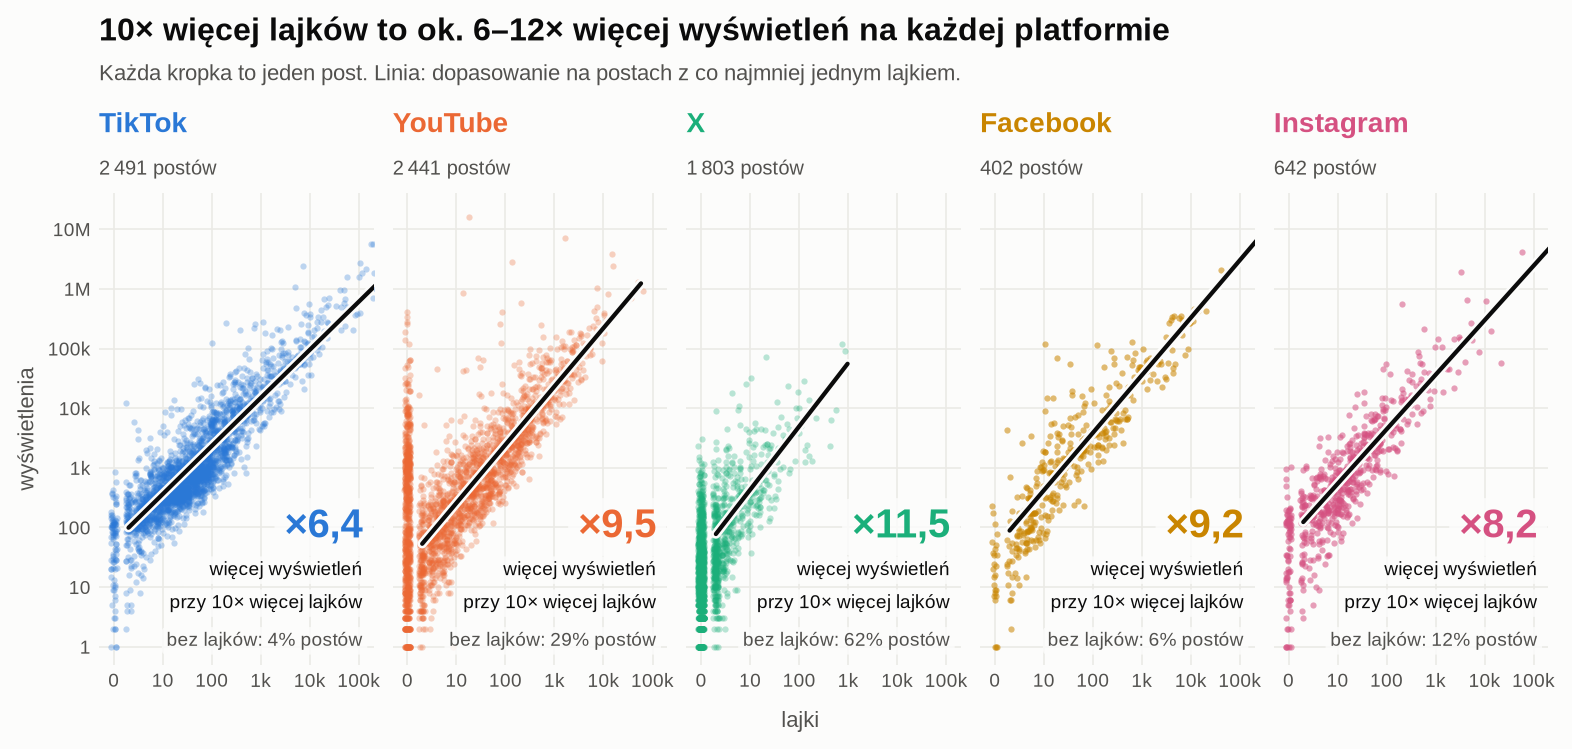
\includegraphics[width=\textwidth,height=.8\textheight,keepaspectratio]{fig/data_overview_pl.png}
\end{frame}

% ------------------------------------------------------------
\section{Metoda}

\begin{frame}{Dwa scenariusze}
\begin{columns}[T]
\column{.48\textwidth}
\begin{block}{Na tej samej platformie}
TikTok, YouTube, X\\[2pt]
CatBoost na obserwujących, reakcjach i flagach braków\\[2pt]
ocena na \alert{markach i autorach}, których model nie widział
\end{block}
\column{.48\textwidth}
\begin{block}{Poza platformą}
Facebook, Instagram (+ Stack Exchange)\\[2pt]
regresja liniowa (ridge) na $\log$ lajków i komentarzy\\[2pt]
uczona \alert{tylko na X i YouTube}, 0 postów z platformy docelowej
\end{block}
\end{columns}
\vspace{8pt}
\begin{center}
Błąd: MAE na $\log_{10}$ wyświetleń, podawany jako \alert{typowy błąd $10^{\text{MAE}}$}\\
{\small \x{2} = oszacowanie zwykle 2 razy za duże albo za małe}
\end{center}
\end{frame}

% ------------------------------------------------------------
\section{Wyniki}

\begin{frame}{Główne wyniki: o ile mylimy się na pojedynczym poście}
\centering\small
\begin{tabular}{lllccc}
\toprule
 & & Posty / marki & \textbf{Nasz błąd} (MAE) & W granicach \x{2} & Stała mediana \\
\midrule
\multirow{3}{*}{\shortstack[l]{Ta sama\\platforma}} & TikTok & 2\,491 / 266 & \xb{1,87} (0,273) & 67\% & \x{4,60} \\
 & YouTube & 2\,441 / 273 & \xb{2,90} (0,462) & 43\% & \x{8,77} \\
 & X & 1\,803 / 252 & \xb{3,03} (0,482) & 40\% & \x{4,63} \\
\midrule
\multirow{2}{*}{\shortstack[l]{Poza\\platformą}} & Facebook & 402 / 20 & \xb{2,43} (0,385) & 53\% & \x{19,87} \\
 & Instagram & 642 / 11 & \xb{2,72} (0,435) & 40\% & \x{8,69} \\
\bottomrule
\end{tabular}
\vspace{8pt}
\begin{itemize}
  \item Facebook: tyle samo, co ridge uczony na samym Facebooku (\x{2,42})
  \item Instagram: gorzej niż ridge uczony na Instagramie (\x{2,41}); 72\% rolek niedoszacowanych
\end{itemize}
\end{frame}

\begin{frame}{Oszacowane a prawdziwe wyświetlenia}
\centering
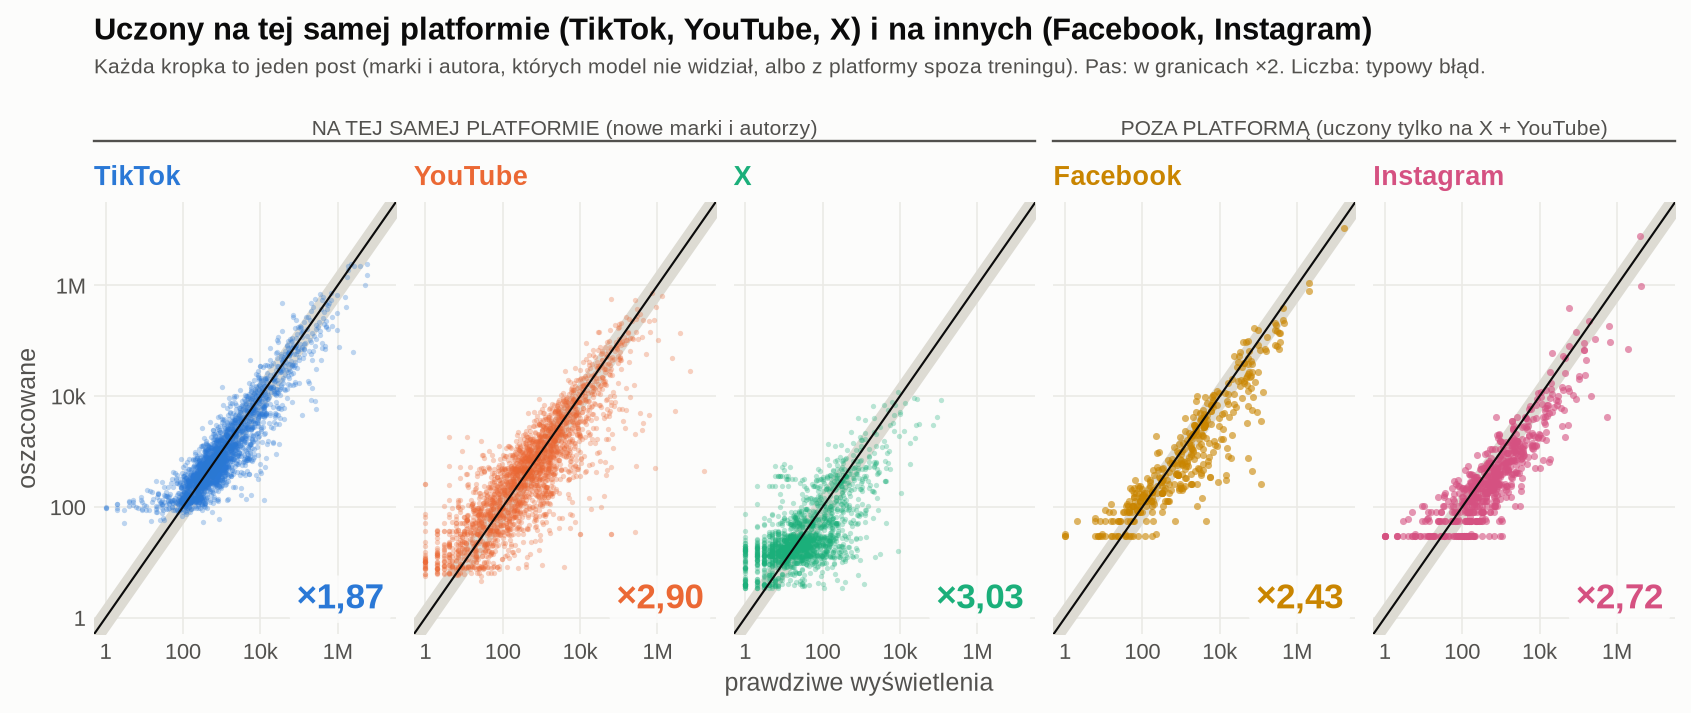
\includegraphics[width=\textwidth,height=.82\textheight,keepaspectratio]{fig/preprint_main_pl.png}
\end{frame}

\begin{frame}{Regresja a stały mnożnik lajków (ok. 25 wyświetleń na lajk)}
\centering\footnotesize\setlength{\tabcolsep}{4pt}
\begin{tabular}{llcccc}
\toprule
Cel & Źródło & Regresja & Mnożnik lajków & Różnica MAE [95\% CI] & Mediana źródła \\
\midrule
TikTok & X + YT & \xb{2,05} & \x{2,22} & $-$0,034 [$-$0,038; $-$0,029] & \x{11,0} \\
YouTube & pozostałe 4 & \x{4,08} & \x{4,03} & +0,004 [0,000; 0,009] & \x{8,9} \\
X & pozostałe 4 & \x{4,37} & \xb{3,45} & +0,103 [0,084; 0,120] & \x{22,1} \\
Facebook & X + YT & \x{2,43} & \x{2,42} & +0,002 [$-$0,017; 0,022] & \x{19,9} \\
Instagram & X + YT & \xb{2,72} & \x{2,94} & $-$0,034 [$-$0,047; $-$0,020] & \x{8,7} \\
Stack Exchange & X + YT & \x{3,14} & \x{5,33} & $-$0,229 [$-$0,240; $-$0,207] & \xb{2,1} \\
\bottomrule
\end{tabular}
\vspace{8pt}
\begin{itemize}
  \item Regresja lepsza na 3, bez wyraźnej różnicy na 2 (FB, YT), gorsza na X (62\% postów bez lajka)
  \item Obie metody 2--8 razy lepsze od mediany na platformach z filmami
\end{itemize}
\end{frame}

% ------------------------------------------------------------
\section{Przeniesienie między platformami}

\begin{frame}{Każda platforma jako ,,ukryta'': różne zestawy treningowe}
\centering\scriptsize
\setlength{\tabcolsep}{5pt}\renewcommand{\arraystretch}{1.05}
\begin{tabular}{l|ccccc|c}
\toprule
Trening na & TikTok & YouTube & X & Facebook & Instagram & Stack Exchange \\
\midrule
\textit{ridge, ta sama platforma} & \cellcolor[HTML]{DDEBFC}1,99 & \cellcolor[HTML]{5A95DF}4,15 & \cellcolor[HTML]{A3C8F2}3,30 & \cellcolor[HTML]{DDEBFC}2,42 & \cellcolor[HTML]{DDEBFC}2,41 & \cellcolor[HTML]{DDEBFC}1,77 \\ \midrule
YT & \cellcolor[HTML]{DDEBFC}\textbf{2,00} & \cellcolor[HTML]{EEEDEA}{\color{black!35}trening} & \cellcolor[HTML]{3779CF}\textcolor{white}{4,64} & \cellcolor[HTML]{C3DCF8}2,72 & \cellcolor[HTML]{C3DCF8}2,63 & \cellcolor[HTML]{DDEBFC}1,87 \\
FB & \cellcolor[HTML]{DDEBFC}2,30 & \cellcolor[HTML]{3779CF}\textcolor{white}{4,26} & \cellcolor[HTML]{7FB0EA}\textbf{3,60} & \cellcolor[HTML]{EEEDEA}{\color{black!35}trening} & \cellcolor[HTML]{C3DCF8}\textbf{2,47} & \cellcolor[HTML]{A3C8F2}3,32 \\
IG & \cellcolor[HTML]{C3DCF8}2,46 & \cellcolor[HTML]{3779CF}\textcolor{white}{4,50} & \cellcolor[HTML]{5A95DF}4,06 & \cellcolor[HTML]{C3DCF8}2,48 & \cellcolor[HTML]{EEEDEA}{\color{black!35}trening} & \cellcolor[HTML]{C3DCF8}2,46 \\
TT & \cellcolor[HTML]{EEEDEA}{\color{black!35}trening} & \cellcolor[HTML]{5A95DF}\textbf{4,07} & \cellcolor[HTML]{5A95DF}4,15 & \cellcolor[HTML]{C3DCF8}2,61 & \cellcolor[HTML]{C3DCF8}2,59 & \cellcolor[HTML]{DDEBFC}2,41 \\
X & \cellcolor[HTML]{7FB0EA}3,38 & \cellcolor[HTML]{184A8C}\textcolor{white}{5,52} & \cellcolor[HTML]{EEEDEA}{\color{black!35}trening} & \cellcolor[HTML]{A3C8F2}3,07 & \cellcolor[HTML]{C3DCF8}2,74 & \cellcolor[HTML]{3779CF}\textcolor{white}{4,50} \\
\midrule
X + YT & \cellcolor[HTML]{DDEBFC}2,05 & \cellcolor[HTML]{EEEDEA}{\color{black!35}trening} & \cellcolor[HTML]{EEEDEA}{\color{black!35}trening} & \cellcolor[HTML]{DDEBFC}\textbf{2,43} & \cellcolor[HTML]{C3DCF8}2,72 & \cellcolor[HTML]{A3C8F2}3,14 \\
\midrule
TT + YT + X & \cellcolor[HTML]{EEEDEA}{\color{black!35}trening} & \cellcolor[HTML]{EEEDEA}{\color{black!35}trening} & \cellcolor[HTML]{EEEDEA}{\color{black!35}trening} & \cellcolor[HTML]{C3DCF8}2,49 & \cellcolor[HTML]{C3DCF8}2,69 & \cellcolor[HTML]{A3C8F2}3,08 \\
\midrule
YT + X + FB + IG & \cellcolor[HTML]{DDEBFC}2,12 & \cellcolor[HTML]{EEEDEA}{\color{black!35}trening} & \cellcolor[HTML]{EEEDEA}{\color{black!35}trening} & \cellcolor[HTML]{EEEDEA}{\color{black!35}trening} & \cellcolor[HTML]{EEEDEA}{\color{black!35}trening} & \cellcolor[HTML]{A3C8F2}3,25 \\
TT + YT + X + IG & \cellcolor[HTML]{EEEDEA}{\color{black!35}trening} & \cellcolor[HTML]{EEEDEA}{\color{black!35}trening} & \cellcolor[HTML]{EEEDEA}{\color{black!35}trening} & \cellcolor[HTML]{C3DCF8}2,46 & \cellcolor[HTML]{EEEDEA}{\color{black!35}trening} & \cellcolor[HTML]{A3C8F2}3,07 \\
TT + YT + X + FB & \cellcolor[HTML]{EEEDEA}{\color{black!35}trening} & \cellcolor[HTML]{EEEDEA}{\color{black!35}trening} & \cellcolor[HTML]{EEEDEA}{\color{black!35}trening} & \cellcolor[HTML]{EEEDEA}{\color{black!35}trening} & \cellcolor[HTML]{C3DCF8}2,66 & \cellcolor[HTML]{A3C8F2}3,08 \\
TT + X + FB + IG & \cellcolor[HTML]{EEEDEA}{\color{black!35}trening} & \cellcolor[HTML]{5A95DF}4,08 & \cellcolor[HTML]{EEEDEA}{\color{black!35}trening} & \cellcolor[HTML]{EEEDEA}{\color{black!35}trening} & \cellcolor[HTML]{EEEDEA}{\color{black!35}trening} & \cellcolor[HTML]{3779CF}\textcolor{white}{4,24} \\
TT + YT + FB + IG & \cellcolor[HTML]{EEEDEA}{\color{black!35}trening} & \cellcolor[HTML]{EEEDEA}{\color{black!35}trening} & \cellcolor[HTML]{3779CF}\textcolor{white}{4,37} & \cellcolor[HTML]{EEEDEA}{\color{black!35}trening} & \cellcolor[HTML]{EEEDEA}{\color{black!35}trening} & \cellcolor[HTML]{DDEBFC}2,11 \\
\bottomrule
\end{tabular}

\sub{Typowy błąd (\x{}). Szare: platforma w treningu. Pierwszy wiersz: ridge uczony na platformie testowej.
Mediana po wszystkich 15 zestawach bez celu: FB \x{2,58}, IG \x{2,65}, czyli wynik nie zależy od wyboru X + YT.}
\end{frame}

\begin{frame}{Trzy przedziały zamiast liczby}
\centering
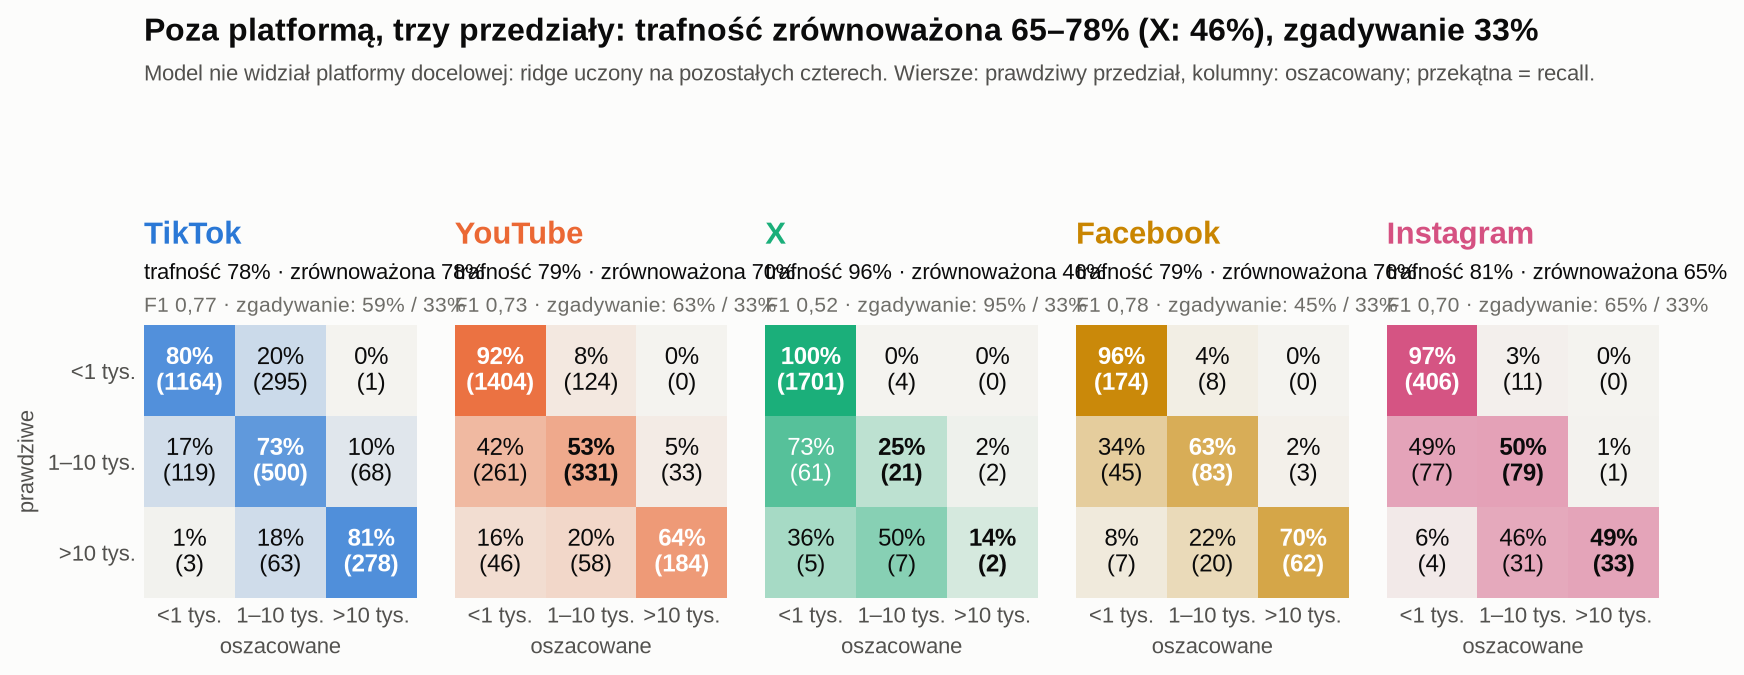
\includegraphics[width=\textwidth,height=.8\textheight,keepaspectratio]{fig/preprint_bins_pl.png}
\end{frame}

\begin{frame}{Czego model potrzebuje}
\centering
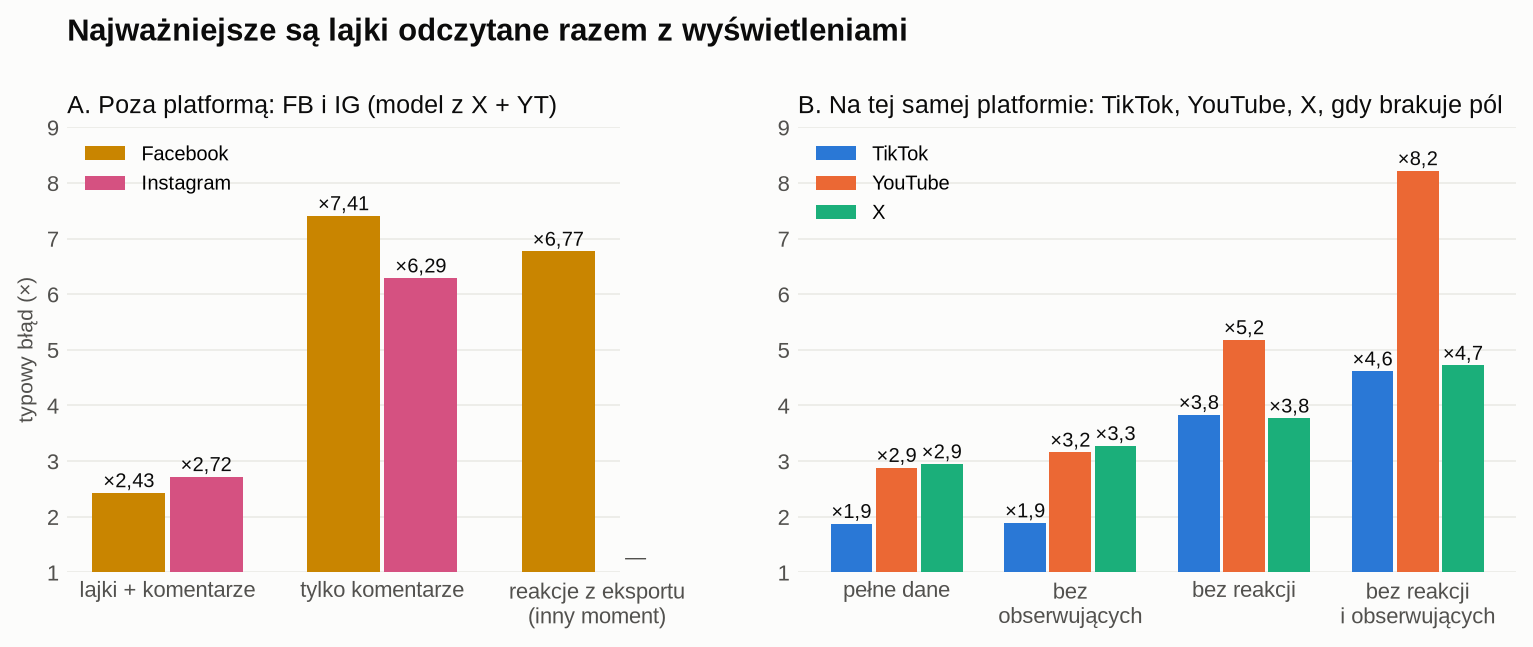
\includegraphics[width=\textwidth,height=.8\textheight,keepaspectratio]{fig/preprint_needs_pl.png}
\sub{Kluczowe: lajki odczytane w tej samej chwili co wyświetlenia. Same komentarze: \x{6,3}--\x{7,4}.}
\end{frame}

\begin{frame}{Szósta platforma: Stack Exchange (538 pytań, 48 marek)}
\centering
\begin{tabular}{lcc}
\toprule
Metoda & Typowy błąd & Spearman \\
\midrule
ridge z X + YouTube & \x{3,14} & 0,57 \\
stały mnożnik lajków (upvote = lajk) & \x{5,33} & \\
mediana X + YouTube & \x{2,10} & \\
mediana samego Stack Exchange & \x{1,96} & \\
ridge uczony na Stack Exchange & \x{1,77} & 0,57 \\
\bottomrule
\end{tabular}
\vspace{10pt}
\begin{itemize}
  \item Przenosi się \alert{kolejność}, nie poziom: 96\% pytań niedoszacowanych
  \item Stosunek wyświetleń do reakcji przenosi się między serwisami z filmami, nie na serwis Q\&A
\end{itemize}
\end{frame}

% ------------------------------------------------------------
\section{Porównanie metod}

\begin{frame}{Na tej samej platformie prawie wszystkie modele są równe}
\centering\small
\begin{tabular}{lccc}
\toprule
Model & TikTok & YouTube & X \\
\midrule
mediana wyświetleń platformy & \x{4,60} & \x{8,79} & \x{4,65} \\
stały mnożnik liczby obserwujących & \x{8,30} & \x{7,16} & \x{7,57} \\
stały mnożnik lajków & \x{2,23} & \x{4,06} & \x{3,63} \\
\midrule
regresja liniowa (ridge) & \x{1,89} & \x{3,51} & \x{3,07} \\
las losowy & \x{1,88} & \x{2,90} & \x{2,97} \\
XGBoost & \x{1,87} & \x{2,82} & \x{2,93} \\
\textbf{CatBoost (model końcowy)} & \x{1,87} & \x{2,83} & \x{2,95} \\
perceptron wielowarstwowy (MLP) & \x{1,89} & \x{2,84} & \x{3,00} \\
TabPFN v2 & \x{1,85} & \x{2,77} & \x{2,92} \\
\midrule
stos wszystkich rodzin & \x{1,82} & \x{2,66} & \x{2,76} \\
\bottomrule
\end{tabular}
\sub{Walidacja po markach, 40 ustawień na fałd. 95\% CI CatBoost: $\pm$0,012--0,021 MAE.
Ponad 20 dodatkowych źródeł (tekst, etykiety AI, grafy, Wikipedia) poprawia błąd najwyżej \x{1,04}.}
\end{frame}

% ------------------------------------------------------------
\section{Zastosowania}

\begin{frame}{Alert o wybiciu, ranking marek, wartość medialna}
\centering
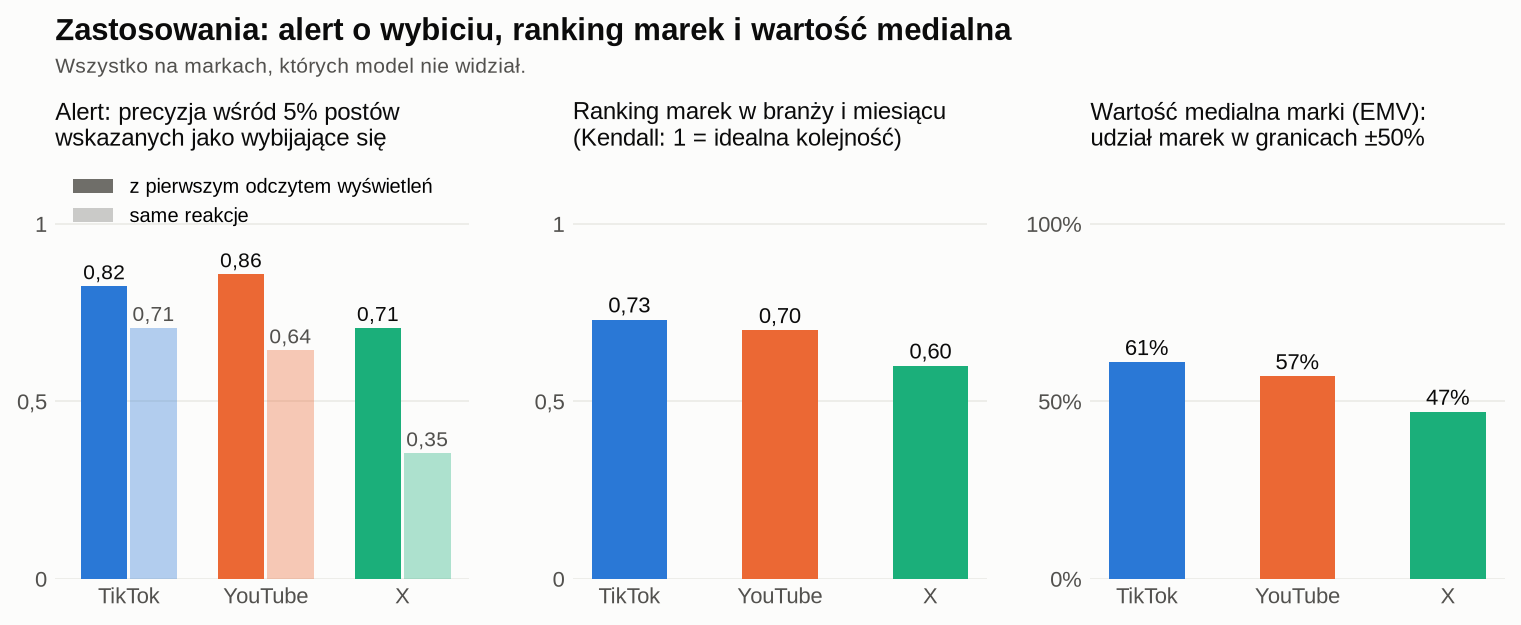
\includegraphics[width=\textwidth,height=.8\textheight,keepaspectratio]{fig/preprint_side_pl.png}
\end{frame}

\begin{frame}{Kolumna zasięgu w eksporcie a nasze oszacowanie (X)}
\centering
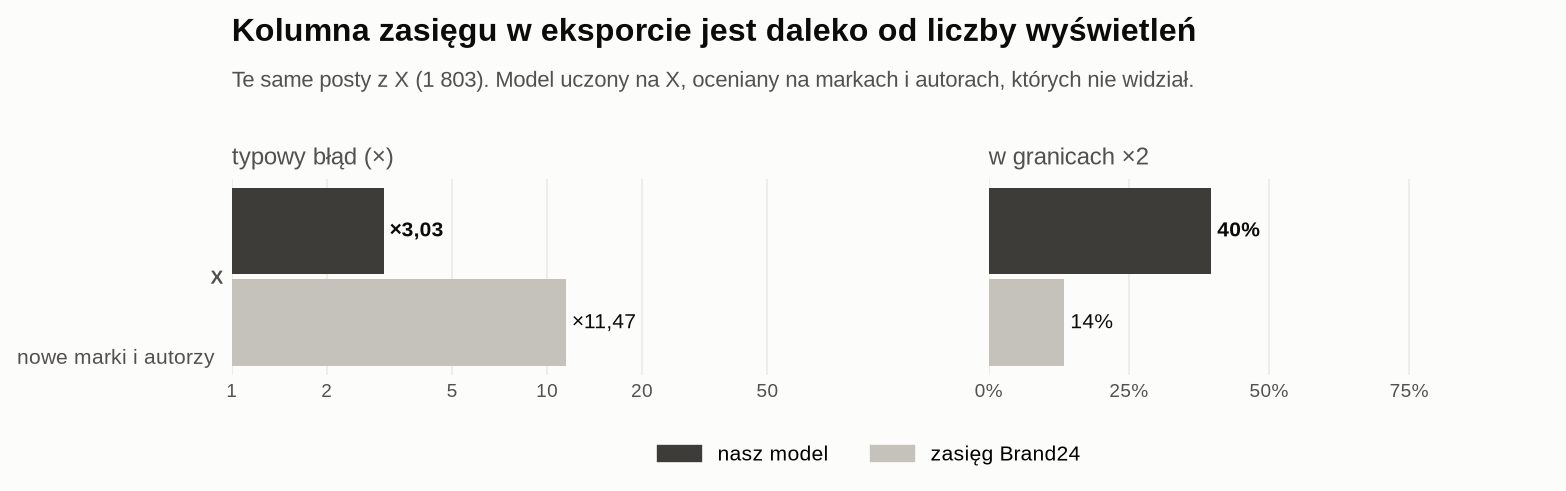
\includegraphics[width=\textwidth,height=.7\textheight,keepaspectratio]{fig/final_compare_pl.png}
\sub{Zasięg to inna miara niż wyświetlenia: pokazujemy, jak daleko od wyświetleń jest liczba, którą klient dostaje dziś.}
\end{frame}

% ------------------------------------------------------------
\section{Ograniczenia}

\begin{frame}{Ograniczenia}
\begin{columns}[T]
\column{.48\textwidth}
\begin{block}{Mało marek}
FB: 20, IG: 11. Bez 3 największych: \x{2,89} i \x{2,96}.
Jedna marka: \x{1,5}--\x{6,2} (FB)
\end{block}
\begin{block}{Wiek odczytu}
Eksport: 23 dni, nasz odczyt FB/IG: 310--334 dni
\end{block}
\begin{block}{Wybór postów}
Tylko dostępne filmy i rolki; bez rolek z ukrytymi lajkami
\end{block}
\column{.48\textwidth}
\begin{block}{X}
Regresja gorsza od stałego mnożnika; 62\% postów bez lajka
\end{block}
\begin{block}{Wzmianki nie o marce}
6,7\% bez nazwy marki w tekście
\end{block}
\begin{block}{Korelacja, nie przyczynowość}
Opisujemy związki, nie przyczyny
\end{block}
\end{columns}
\end{frame}

% ------------------------------------------------------------
\section{Wnioski}

\begin{frame}{Wnioski}
\begin{enumerate}
  \item Prosta regresja na lajkach i komentarzach, uczona tylko na X i YouTube, szacuje wyświetlenia FB z błędem
        \alert{\x{2,43}}, a IG z błędem \alert{\x{2,72}}; mediana myli się \x{9}--\x{20}
  \item W praktyce przenosi się \alert{stosunek wyświetleń do lajków}; warunek: reakcje odczytane razem z wyświetleniami
  \item Nie działa wszędzie: X gorszy od stałego mnożnika, Stack Exchange tylko kolejność
\end{enumerate}
\vspace{6pt}
\begin{block}{Rekomendacja dla dostawcy monitoringu}
Odczytywać reakcje razem z wyświetleniami, zapisywać braki jako braki, robić drugi odczyt wyświetleń
\end{block}
\end{frame}

\end{document}
